%%%%%%%%%%%%%%%%%%%%%%%%%%%%%%%%%%%%%%%%%
% Beamer Presentation
% LaTeX Template
% Version 1.0 (10/11/12)
%
% This template has been downloaded from:
% http://www.LaTeXTemplates.com
%
% License:
% CC BY-NC-SA 3.0 (http://creativecommons.org/licenses/by-nc-sa/3.0/)
%
%%%%%%%%%%%%%%%%%%%%%%%%%%%%%%%%%%%%%%%%%

%----------------------------------------------------------------------------------------
%	PACKAGES AND THEMES
%----------------------------------------------------------------------------------------

\documentclass{beamer}
\mode<presentation> {

% The Beamer class comes with a number of default slide themes
% which change the colors and layouts of slides. Below this is a list
% of all the themes, uncomment each in turn to see what they look like.

%\usetheme{default}
%\usetheme{AnnArbor}
% %\usetheme{Antibes}
%\usetheme{Bergen}
%\usetheme{Berkeley}
%\usetheme{Berlin}
%\usetheme{Boadilla}
%\usetheme{CambridgeUS}
%\usetheme{Copenhagen}
%\usetheme{Darmstadt}
%\usetheme{Dresden}
%\usetheme{Frankfurt}
%\usetheme{Goettingen}
%\usetheme{Hannover}
%\usetheme{Ilmenau}
%\usetheme{JuanLesPins}
%\usetheme{Luebeck}
\usetheme{Madrid} %%%%
%\usetheme{Malmoe}
%\usetheme{Marburg}
%\usetheme{Montpellier}
%\usetheme{PaloAlto}
%\usetheme{Pittsburgh}
%\usetheme{Rochester}
%\usetheme{Singapore}
%\usetheme{Szeged}
%\usetheme{Warsaw}

% As well as themes, the Beamer class has a number of color themes
% for any slide theme. Uncomment each of these in turn to see how it
% changes the colors of your current slide theme.

%\usecolortheme{albatross}
%\usecolortheme{beaver}
%\usecolortheme{beetle}
%\usecolortheme{crane}
%\usecolortheme{dolphin}
%\usecolortheme{dove}
%\usecolortheme{fly}
%\usecolortheme{lily}
%\usecolortheme{orchid}
%\usecolortheme{rose}
%\usecolortheme{seagull}
%\usecolortheme{seahorse}
%\usecolortheme{whale}
%\usecolortheme{wolverine}

%\setbeamertemplate{footline} % To remove the footer line in all slides uncomment this line
%\setbeamertemplate{footline}[page number] % To replace the footer line in all slides with a simple slide count uncomment this line

%\setbeamertemplate{navigation symbols}{} % To remove the navigation symbols from the bottom of all slides uncomment this line
}

\usepackage{graphicx} % Allows including images
\usepackage{graphics}
\usepackage{booktabs} % Allows the use of \toprule, \midrule and \bottomrule in tables
\usepackage[english, french]{babel}  %support francais et anglais
\usepackage[utf8]{inputenc}
%\bibliographystyle{plainnat}
%\bibliography{cdansereau}


%----------------------------------------------------------------------------------------
%	TITLE PAGE
%----------------------------------------------------------------------------------------

\title[Schizophrenia classification]{Schizophrenia classification using \\multi-scale functional connectivity } % The short title appears at the bottom of every slide, the full title is only on the title page

\author{Christian Dansereau} % Your name
\institute[DIRO] % Your institution as it will appear on the bottom of every slide, may be shorthand to save space
{
Université de Montréal \\ % Your institution for the title page
\medskip
%\textit{john@smith.com} % Your email address
}
\date{28 Avril 2015} % Date, can be changed to a custom date

\begin{document}

\begin{frame}
\titlepage % Print the title page as the first slide
\end{frame}

\begin{frame}
\frametitle{Overview} % Table of contents slide, comment this block out to remove it
\tableofcontents % Throughout your presentation, if you choose to use \section{} and \subsection{} commands, these will automatically be printed on this slide as an overview of your presentation
\end{frame}

%----------------------------------------------------------------------------------------
%	PRESENTATION SLIDES
%----------------------------------------------------------------------------------------

%------------------------------------------------
\section{Contexte général} 
%------------------------------------------------

%------------------------------------------------
%\subsection{Imagerie par résonance magnétique fonctionnelle} 
%------------------------------------------------

\begin{frame}
\frametitle{Imagerie par résonance magnétique (IRM)}
\begin{figure}
\begin{center}
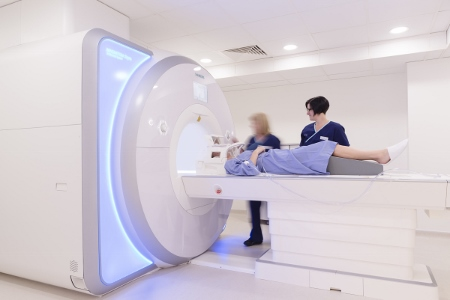
\includegraphics[width=0.7\linewidth]{../figures/scanner.jpg}
\end{center}
\end{figure}
\end{frame}


\begin{frame}
\frametitle{IRM fonctionnelle (IRMf)}
\begin{figure}[H]
\begin{center}
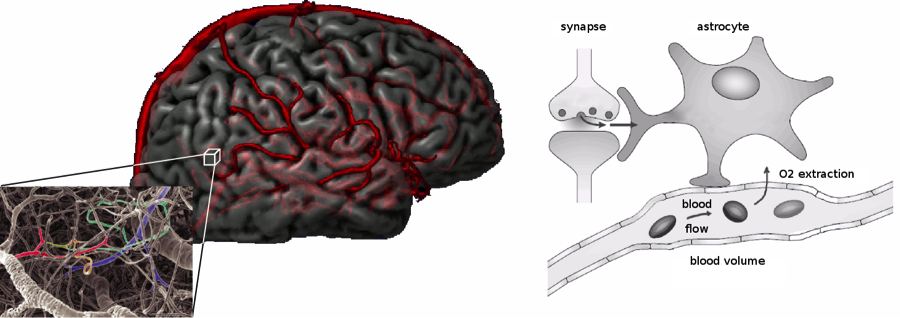
\includegraphics[width=\linewidth]{../figures/bold.png}
\end{center}
\tiny{Adapté de Heeger 2002.}
\end{figure}
\end{frame}

%------------------------------------------------
%\subsection{Prétraitement} 
%------------------------------------------------

\frame{\sectionpage}

\begin{frame}
\frametitle{Connectome}
\begin{figure}
\begin{center}
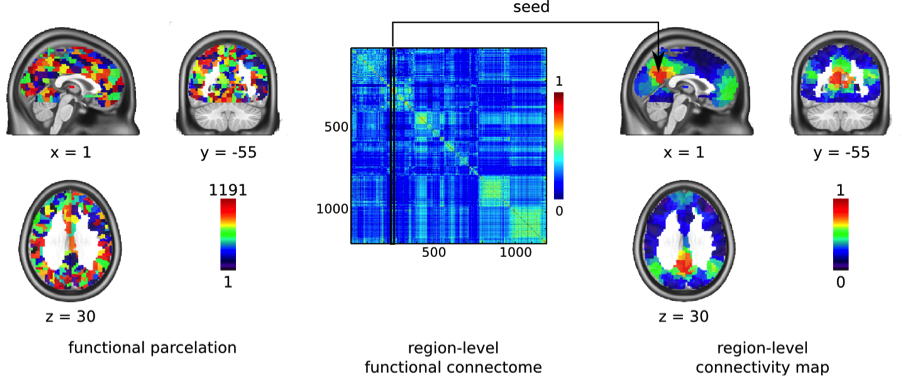
\includegraphics[scale=0.8]{../figures/connectome.png}
\end{center}
\tiny{(``Neuroimaging Analysis Kit'' (NIAK) \footnote{\url{http://www.nitrc.org/projects/niak/}}).}
\label{fig_motion_estimation}
\end{figure}
\end{frame}


\begin{frame}
\frametitle{Multiscale connectomes}
\begin{figure}
\begin{center}
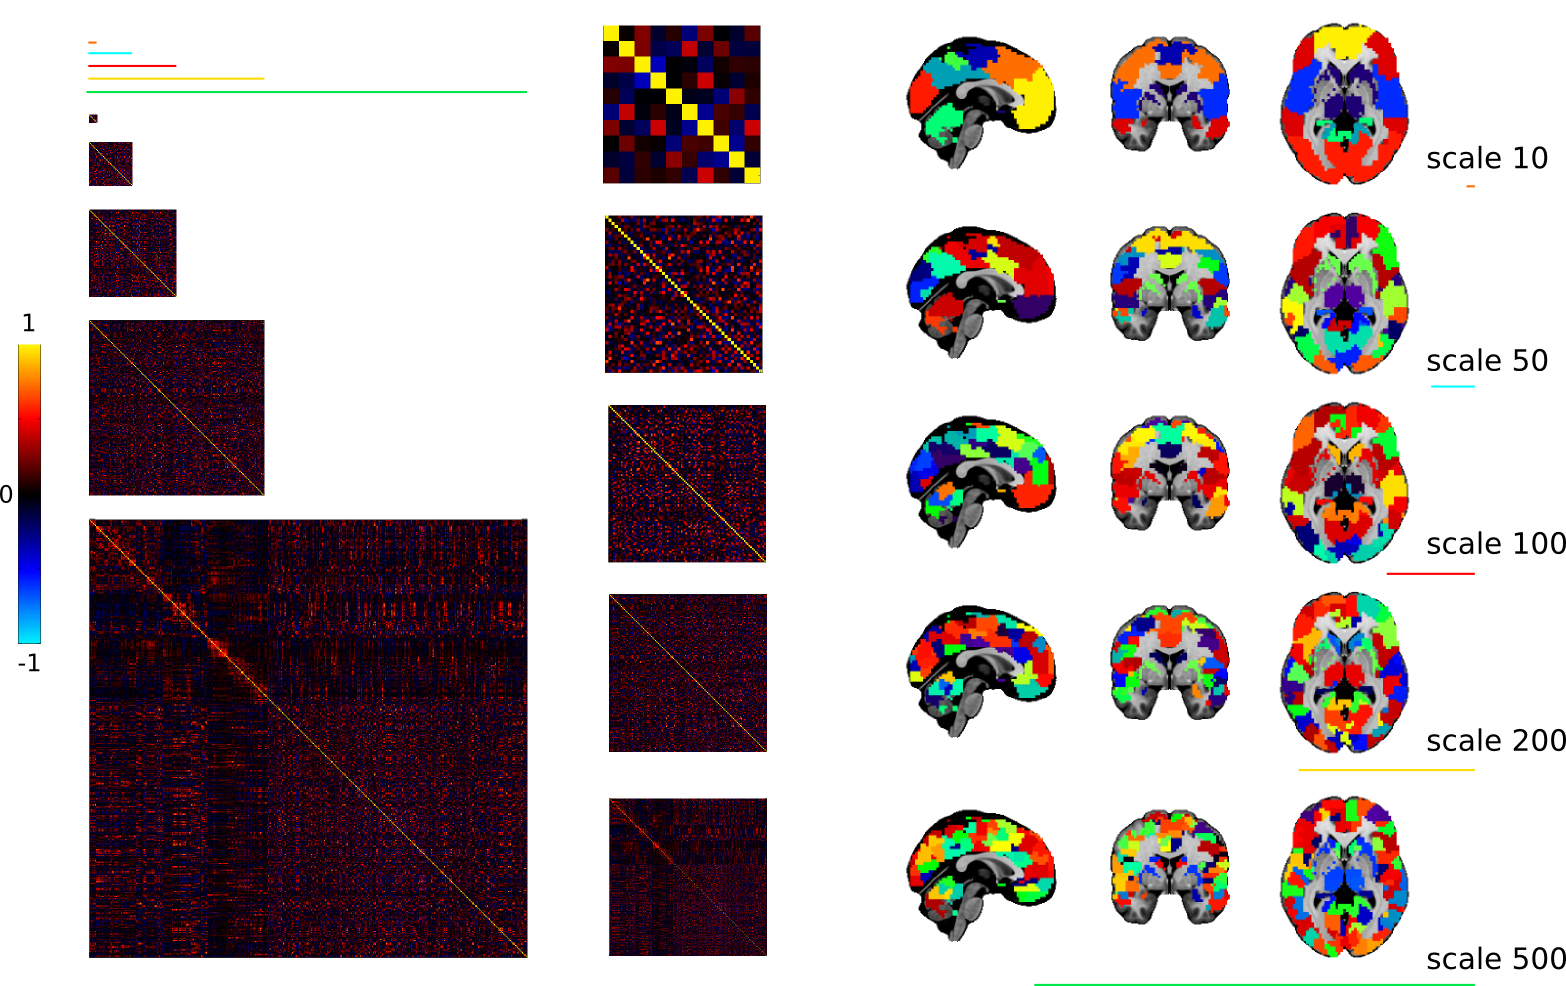
\includegraphics[scale=0.5]{../figures/fig_connectome_multiscale.png}
\end{center}
\tiny{Multiscale connectomes.}
\label{fig_multiscale}
\end{figure}
\end{frame}


\begin{frame}
\frametitle{Multiscale connectomes COBRE}
\begin{figure}
\begin{center}
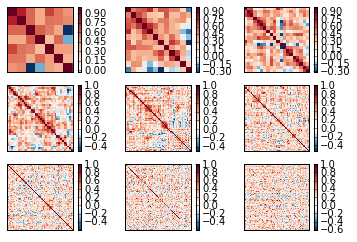
\includegraphics[scale=0.9]{../figures/connectome3x3.png}
\end{center}
\tiny{Multiscale connectomes COBRE (7, 12, 20, 36, 64, 122, 197, 325 and 444).}
\label{fig_multiscale_cobre}
\end{figure}
\end{frame}


\frame{
\frametitle{Jeux de données}
Ce projet provient de l’agrégation de plusieurs jeux de données (5 études différentes)
\hfill\break
ADNI2 et 4 études basées à Montréal (total: 313 sujets)
\begin{itemize}
\item 126 CNE participants (51M, âge = 57-94)
\item 133 pMCI (70M, âge = 55-89) 
\item 54 pDAT (22M, âge = 55-88)
\end{itemize}
\hfill\break
Jeux de données de référence: ``1000 functional connectome project''
\begin{itemize}
\item 355 jeunes adultes sains (CNY) (150M, âge = 18-46)
\end{itemize}
}


%------------------------------------------------
\section{Méthod}
%------------------------------------------------



\begin{frame}
\frametitle{Correction des artefacts de mouvement}
Les mouvements de la tête sont inévitables et présentent l’un des plus grands problèmes en IRMf.
\hfill\break
\begin{itemize}
\item Possibilité de réaligner les déplacements de la tête.
\item Ne corrige pas les artefacts induits dans le signal par des inhomogénéités du champ magnétique.
\item Le mouvement est plus important/fréquent chez les populations âgées. 
\end{itemize}
\end{frame}

%------------------------------------------------
\section{Résultats}
%------------------------------------------------

%------------------------------------------------
\section{Conclusion}
%------------------------------------------------

%----------------------------------------------------------------------------------------

\begin{frame}
\Huge{\centerline{Merci}}
\end{frame}

%----------------------------------------------------------------------------------------


\end{document} 